\documentclass{article}


% if you need to pass options to natbib, use, e.g.:
%     \PassOptionsToPackage{numbers, compress}{natbib}
% before loading neurips_2023


% ready for submission
\usepackage[preprint]{neurips_2023}


% to compile a preprint version, e.g., for submission to arXiv, add add the
% [preprint] option:
%     \usepackage[preprint]{neurips_2023}


% to compile a camera-ready version, add the [final] option, e.g.:
%     \usepackage[final]{neurips_2023}


% to avoid loading the natbib package, add option nonatbib:
%    \usepackage[nonatbib]{neurips_2023}


\usepackage[utf8]{inputenc} % allow utf-8 input
\usepackage[T1]{fontenc}    % use 8-bit T1 fonts
\usepackage{hyperref}       % hyperlinks
\usepackage{url}            % simple URL typesetting
\usepackage{booktabs}       % professional-quality tables
\usepackage{amsfonts}       % blackboard math symbols
\usepackage{nicefrac}       % compact symbols for 1/2, etc.
\usepackage{microtype}      % microtypography
\usepackage{xcolor}         % colors

\usepackage{amsmath}
\usepackage{array}
\usepackage{graphicx}
\usepackage{subfigure}

\title{Reinforcement Learning for Car Racing in OpenAI Gym using Double Deep Q-Learning (DDQN)}



% The \author macro works with any number of authors. There are two commands
% used to separate the names and addresses of multiple authors: \And and \AND.
%
% Using \And between authors leaves it to LaTeX to determine where to break the
% lines. Using \AND forces a line break at that point. So, if LaTeX puts 3 of 4
% authors names on the first line, and the last on the second line, try using
% \AND instead of \And before the third author name.


\author{%
  Qi Jiachen \\
  2021533125 \\
  \texttt{qijch@shanghaitech.edu.cn} \\
  % \thanks{Use footnote for providing further information
  %   about author (webpage, alternative address)---\emph{not} for acknowledging
  %   funding agencies.} \\
  % Department of Computer Science\\
  % Cranberry-Lemon University\\
  % Pittsburgh, PA 15213 \\
  % \texttt{hippo@cs.cranberry-lemon.edu} \\
  % examples of more authors
  \And
  Shi Junyan \\
  2021533154 \\
  \texttt{shijy@shanghaitech.edu.cn} \\
  \AND
  Xu Chenhao \\
  2021533119 \\
  % Address \\
  \texttt{xuchh@shanghaitech.edu.cn} \\
  \And
  Zhao Zeyu \\
  2021533136 \\
  % Address \\
  \texttt{zhaozy2@shanghaitech.edu.cn} \\
  \And
  Zhu Yuhang \\
  2021533173 \\
  % Address \\
  \texttt{zhuyh3@shanghaitech.edu.cn} \\
}


\begin{document}


\maketitle


\begin{abstract}
Car racing games hold significant practical importance and present a series of challenging technical problems. This final project endeavors to construct a model utilizing reinforcement learning techniques, specifically Double Q-learning (DDQN), within the OpenAI Gym environment. We establish a reward system and conduct experiments involving image processing and model architectures.

\textbf{GitHub Repository:} \url{https://github.com/Sleepless9/CS181-2023fall}
\end{abstract}

\section{Introduction}

Car racing games can be simulated to replicate real-world scenarios, allowing the definition of various constraints and goals. The original OpenAI Gym's CarRacing problem aimed for the car to traverse all track tiles, rather than completing a full lap. However, this implies that if the car misses some tiles, it will need to run at least one more lap. In this project, we modify the end condition to expedite training and testing, concluding an epoch if the car cannot traverse all tiles and fails to accrue new points within a specified frame limit. This unique end condition aims to encourage the agent to consistently progress on the road, swiftly concluding when yawning—a feature potentially beneficial in the realm of autonomous driving.


\section{Problem Analysis}
% \label{gen_inst}
\subsection{Environment}
In our investigation, we have opted to utilize the \texttt{CarRacing-v0} version environment provided by OpenAI Gym to train our autonomous car agent. The track layout is dynamically generated at the commencement of each simulation, denoted as an "episode". Each state is represented by a 96 $\times$ 96 RGB pixel frame, serving as the sole perceptible information for the agent. This frame offers a top-down perspective of the surroundings, encompassing the current position of the car.

Between consecutive frames, the car is presented with the decision to take an action or maintain its current state. The action space is defined as a combination of steering direction, acceleration (gas), and braking. The numerical values for each component of the action space range between -1 and 1. The complete set of actions is enumerated below:
\renewcommand{\arraystretch}{1.5} % Adjust the row height
\begin{table}[ht!]
  \centering
  \caption{Action Space}
  \begin{tabular}{*{3}{>{\centering\arraybackslash}m{6em}}}
    \hline
    (-1, 1, 0.5) & (0, 1, 0.5) & (1, 1, 0.5) \\
    (-1, 1,  0 ) & (0, 1,  0 ) & (1, 1,  0 ) \\
    (-1, 0, 0.5) & (0, 0, 0.5) & (1, 0, 0.5) \\
    (-1, 0,  0 ) & (0, 0,  0 ) & (1, 0,  0 ) \\
    \hline
  \end{tabular}
\end{table}


\subsection{Grayscale Convertion}
How to perform environment recognition to assist the agent in understanding the environment? 
This problem can lead to many solutions and be applied to the field of autonomous driving.

We choose to do grayscale convertion to help the agent learn about the environment from 
observation. Such a solution is enough to help us complete the recognition in the box2d 
environment, and will not produce too much calculation to drag down the training of the model.

\begin{figure}[ht!]
  \centering
  \caption{Grayscale Convertion Process}
  \subfigure[Observed Image]{
      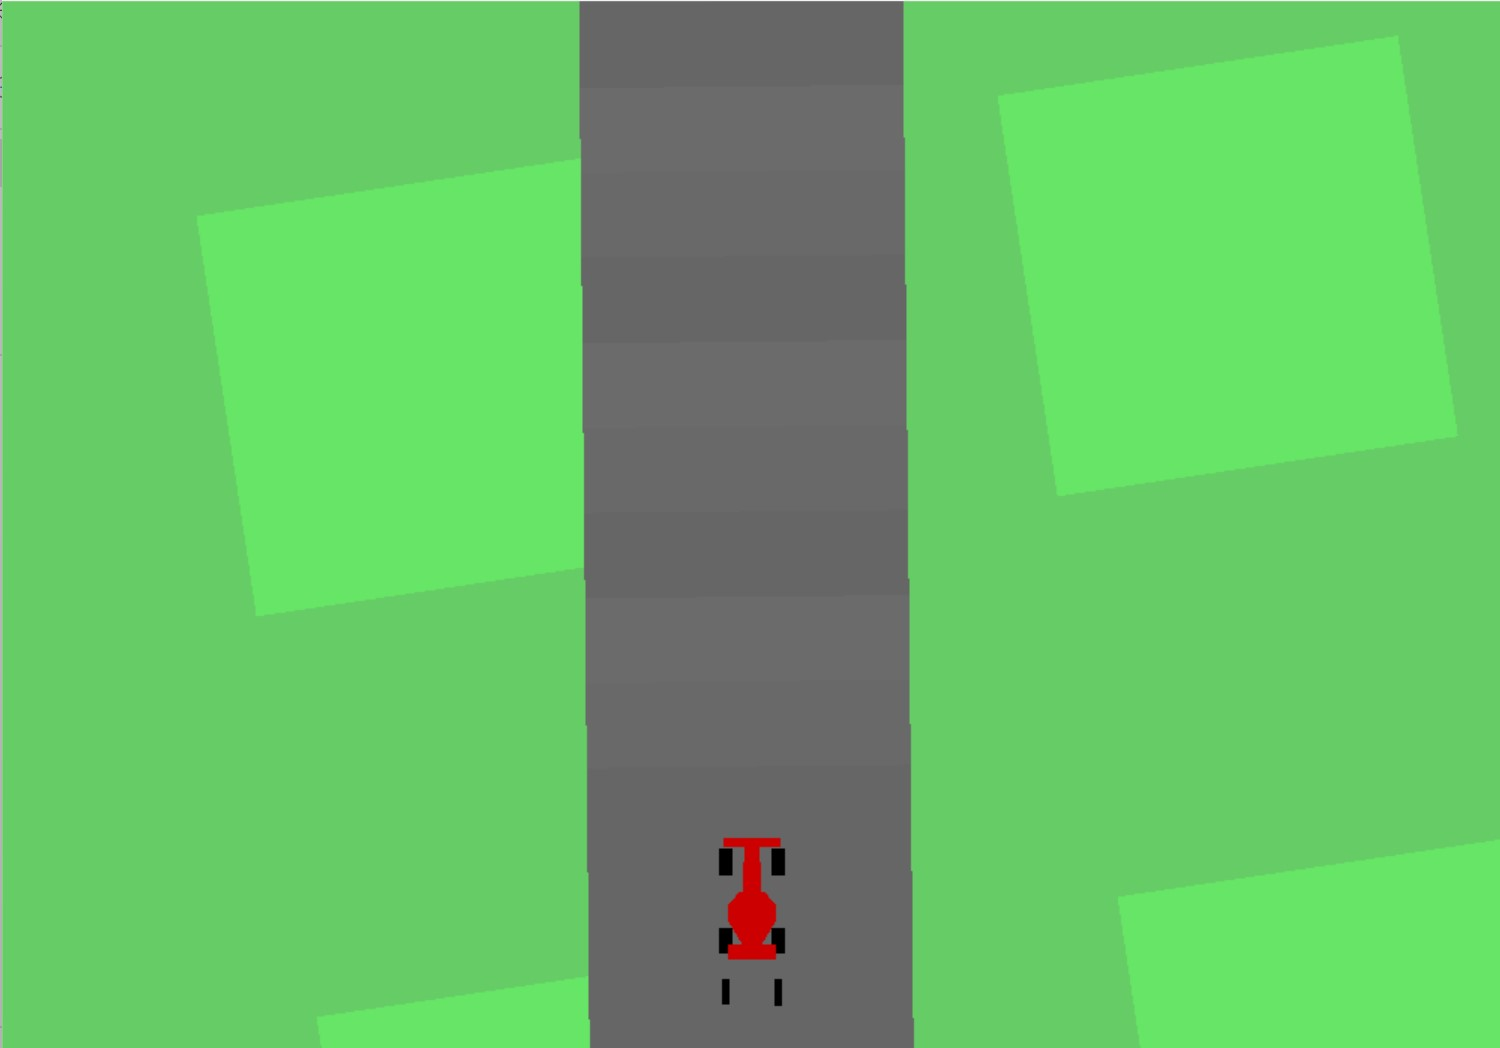
\includegraphics[width=0.3\textwidth]{observe_image.jpg}
      \label{fig:subfig1}
  }
  \subfigure[RGB Image]{
      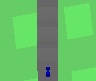
\includegraphics[width=0.3\textwidth]{RGB_image.jpg}
      \label{fig:subfig2}
  }
  \subfigure[Grayscale Image]{
      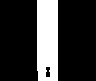
\includegraphics[width=0.3\textwidth]{gray_image.jpg}
      \label{fig:subfig3}
  }
  % \caption{并列的图片}
  % \label{fig:main}
\end{figure}


\section{Related Model}
\label{headings}

\subsection{Double Deep Q Learning (DDQN) Overview}

The conventional Q-learning algorithm often encounters the challenge of overestimating Q-values. Following our team's initial evaluation of Q-learning's efficacy, we introduced the Double Deep Q Learning (DDQN) algorithm, particularly tailored for addressing challenges in dynamic environments like car racing games. DDQN extends the original DQN algorithm by incorporating two neural networks (the main network and the target network) to alleviate the issue of Q-value overestimation.

In the update process, DDQN leverages the target network to compute the Q-value for the subsequent state \(s'\) and subsequently selects the optimal action using the main network. This approach plays a crucial role in diminishing instability arising from overestimation, a critical consideration in the context of car racing scenarios. DDQN seamlessly integrates the updating mechanism of Q-learning but employs deep neural networks to estimate Q-values, thereby enhancing its adaptability to challenges in complex environments. The inclusion of a dual-network structure further bolsters the stability of the learning process, making DDQN particularly well-suited for tasks in our navigating car racing environments.

\subsection{Double Q-learning}

We initialize the Q-learning algorithm by setting parameters related to the environment and action space.

\subsubsection{Experience Replay (\texttt{experience})}

When the number of experiences in the experience pool surpasses a certain threshold, the experience replay mechanism comes into play. This involves:

\begin{itemize}
    \item \texttt{store\_transition}: Storing information about the state, action, reward, next state, and whether it's done for each time step into an experience replay buffer.
    \item \texttt{get\_batch}: Once the observed tuple count surpasses a predefined minimum, the model undergoes iterative improvement by sampling a batch of historical experience tuples from the buffer. This batch is then employed to train the model weights in each iteration.
    \item For each experience sample, calculating the target model's Q-value and updating the Main Model's Q-value:
    
    \[
    Q_{main}[a] = \begin{cases}
    R & \text{if the episode is done} \\
    R + \gamma \max_{a'} Q_{target}(s', a'; \theta^-) & \text{otherwise}
    \end{cases}
    \]
        Here, $\theta^-$ represents the parameters of the target network.
    \item \texttt{update\_model}: Updating the model by copying the parameters of the neural network \texttt{self.model} to the target network \texttt{self.target\_model}.
    
\end{itemize}

\subsubsection{Choosing an Action (\texttt{choose\_action})}

In the context of our exploration strategy, the selection of an action \(a_t\) given the current state \(s_t\) involves utilizing the neural network \texttt{self.model} to predict Q-values for each action in the current state. The decision-making process adheres to an epsilon-greedy policy, where the action with the maximum Q-value is chosen with a probability of \(1 - \epsilon\), and a random action is selected with a probability of \(\epsilon\).
The action \(a_t\) is determined by:
\[
a_t = 
\begin{cases} 
\arg \max_{a} Q(s_t, a; \theta) & \text{with probability } 1 - \epsilon \\
\text{random action} & \text{with probability } \epsilon
\end{cases}
\]
To elaborate on our specific setup, our \(\epsilon\) value is initially set to 1.0 during the early stages of training. After each experience, \(\epsilon\) undergoes exponential decay, diminishing with a decay factor of 0.9999. This decay process continues until \(\epsilon\) reaches a minimum value of 0.05. This dynamic adjustment of \(\epsilon\) serves as a mechanism for balancing exploration and exploitation throughout the training iterations.

\subsection{Neural Network Architecture}

The core of our Double Deep Q Learning (DDQN) model resides in its Convolutional Neural Network (CNN). This network is designed to process raw state representations, extracting essential features and translating them into meaningful Q-value estimates. The architecture is summarized in the table below:

\renewcommand{\arraystretch}{1.5} % Adjust the row height
\begin{table}[ht!]
  \centering
  \caption{CNN Architecture}
  \begin{tabular}{|l|l|l|}
    \hline
    Layer & Operation & Parameters \\
    \hline
    Conv1 & \texttt{ReLU(Conv2D)} & Filters=6, Kernel=(7,7), Strides=3 \\
    MaxPool1 &\texttt{MaxPooling2D} & Pool Size=(2,2) \\
    Conv2 & \texttt{ReLU(Conv2D)} & Filters=12, Kernel=(4,4)  \\
    MaxPool2 & \texttt{MaxPooling2D} & Pool Size=(2,2)  \\
    Flatten &\texttt{Flatten} & -  \\
    Dense1 & \texttt{ReLU(Dense)} & Units=216  \\
    Output &\texttt{Dense }& Units=12, Activation="linear" \\
    \hline
  \end{tabular}
\end{table}

Given the inherent strengths of CNN in image processing tasks, we deliberately chose this architecture as the foundation of our DDQN. The inclusion of multiple layers enables the network to capture hierarchical features, enhancing its ability to discern intricate patterns within the input data. This architectural choice, coupled with the model's capacity for learning intricate spatial representations, suggests promising training outcomes. The potential effectiveness of the model's training process can be influenced by the depth of the CNN, allowing it to grasp both low-level and high-level features essential for making informed decisions in the dynamic environment of the car racing game.

During the compilation phase, we employ Huber Loss as the loss function and the Adam optimizer, which further enhances the model's effectiveness in learning Q-values . This strategic combination emphasizes the importance of precise Q-value estimation throughout the DDQN training process.




\section{Approach}
\label{others}

\subsection{Grayscale Convertion}
Get a 96 $\times$ 96 RGB three-color image from the game. Multiply the y-axis by 0.85
to remove the following scores and the status bar of the vehicle to get a complete picture, 
i.e. reduce the number of pixel blocks to be processed. 
Use cv2 to use color segmentation to convert roads into white, lawns and vehicles into black.

\subsection{Training}
We set \texttt{episode\_num} times to loop, and run the game once in each loop.If the game is over or the road cannot be recognized in the image or the totalreward is less than the minimum value or no positive reward is obtained for 100consecutive frames (that is, no blocks are eaten, it is purely a time deduction),the loop ends. Each time, the obtained state is converted from the color stateto a grayscale image, and \texttt{road\_visibility} is obtained from it to ensure thatthe road can be recognized in the image and avoid meaningless training sets.From the obtained grayscale image, the agent finds the optimal action correspondingto the image in the model, and uses the action to run the game to obtain thenext state. The \texttt{skip\_frames} method is used to introduce time continuity andprovide the agent with more information for decision-making.At the same time, we process the reward obtained and set an upper limit for it. Becausewe don't want it to run too fast, so that it will be easily thrown away when turning.Therefore, no matter how fast the car runs, it can only get so many rewards at most, andgoing too fast will result in a low score, which will drive the car to drive rationally.Then convert the resulting new state from the color state to a grayscale image,and update \texttt{road\_visibility}.After that, the old and new status, action, reward, and whether it is completed are storedin the agent, and experience playback is performed. Finally, reward is added to the total.The process would update the agent's action\_value network every 5 cycles.
\subsection{Test}
This part is to load the model from model to agent. Same as training part,We set \texttt{test\_num} times to loop, and run the game once in each loop.If the game ends or the total reward is less than the minimum value or no positivereward is obtained for 300 consecutive frames (that is, no tiless have been traversed, it ispurely a time deduction), the loop ends. Then convert the obtained state fromcolor state to grayscale image each time. From the obtained grayscale image,the agent finds the optimal action corresponding to the image in the model, and usesthe action to run the game to obtain the next state. The \texttt{skip\_frames}method is usedto introduce time continuity and provide the agent with more information for decision-making.After that, the old and new status, action, reward, and whether it is completed are storedin the agent, and experience playback is performed. Later, reward is added to the total.
Finally, calculate the maximum, minimum, average, and variance of the reward obtained, and 
store the data in the ".csv" file.





\clearpage  % 将浮动环境放置在当前页面的最顶部

\begin{figure}[!h]
  \centering
  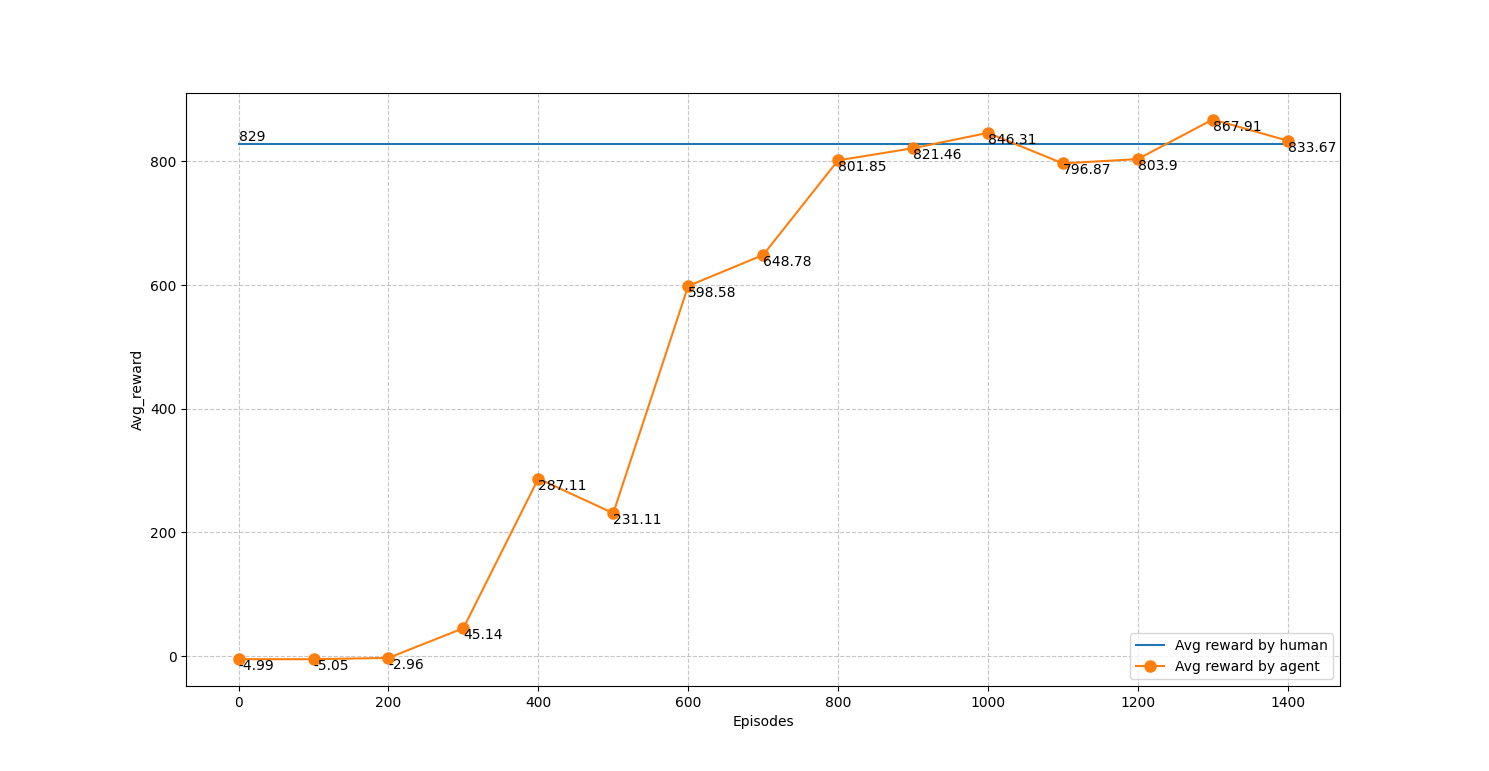
\includegraphics[scale=0.5]{chart.png}
  \caption{Average Rewards}
  \label{figure}
\end{figure}

\section*{References}

\small

[1] andywu0913 (2020). OpenAI-GYM-CarRacing-DQN. GitHub Repository. Retrieved from \url{https://github.com/andywu0913/OpenAI-GYM-CarRacing-DQN}

[2] Gym Library. Car Racing - Gym Document. Retrieved from \url{https://www.gymlibrary.dev/environments/box2d/car_racing/}

[3] van Hasselt, H., Guez, A., \& Silver, D. (2015). Deep Reinforcement Learning with Double Q-learning. Retrieved from \url{https://arxiv.org/abs/1509.06461}

[4] Changmao Li (2019). Challenging On Car Racing Problem from OpenAI Gym.
Retrieved from \url{https://arxiv.org/pdf/1911.04868.pdf}




\end{document}